% =====================================================================
% figure.tex -- schematic of the epidemic-control modelling workflow
%
% Self-contained: compiles with pdflatex as-is.
% Greyscale only; white background; caption below the figure.
% =====================================================================
\documentclass{article}
\usepackage[margin=1in]{geometry}
\usepackage{tikz}
\usetikzlibrary{positioning, shapes.geometric, arrows.meta}

\begin{document}

\begin{figure}[htbp]
  \centering
  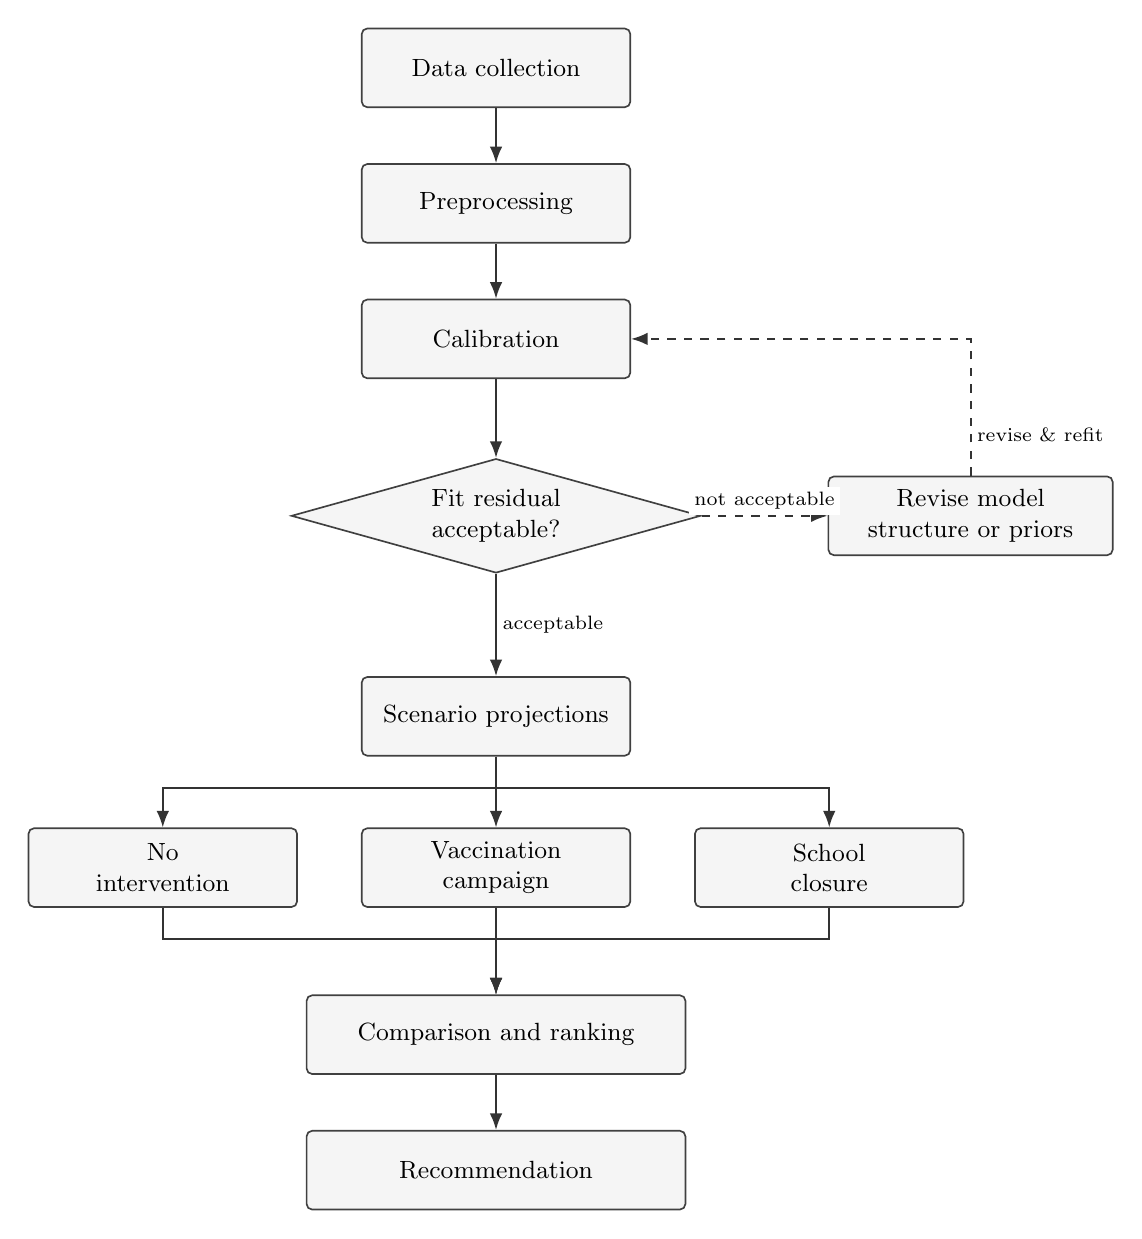
\begin{tikzpicture}[
      proc/.style={rectangle, rounded corners=2pt,
                   draw=black!75, line width=0.6pt,
                   fill=black!4, text width=3.2cm, minimum height=1.0cm,
                   align=center, inner sep=3pt, font=\small},
      dec/.style={diamond, aspect=2.4,
                  draw=black!75, line width=0.6pt,
                  fill=black!4, align=center, inner sep=1pt,
                  minimum width=5.2cm, font=\small},
      flow/.style={draw=black!80, line width=0.7pt,
                   -{Latex[length=2.1mm,width=1.6mm]}},
      retry/.style={draw=black!80, line width=0.7pt, dashed,
                    -{Latex[length=2.1mm,width=1.6mm]}},
      elab/.style={font=\scriptsize, inner sep=2pt, fill=white},
    ]

    % ---- main spine ------------------------------------------------
    \node[proc] (data) {Data collection};
    \node[proc, below=7mm of data] (pre) {Preprocessing};
    \node[proc, below=7mm of pre] (cal) {Calibration};
    \node[dec, below=10mm of cal] (chk) {Fit residual\\acceptable?};

    % ---- revision loop ---------------------------------------------
    \node[proc, text width=3.4cm, right=16mm of chk] (rev)
      {Revise model structure or priors};

    % ---- scenario branch -------------------------------------------
    \node[proc, below=13mm of chk] (proj) {Scenario projections};
    \node[proc, text width=3.2cm, below=9mm of proj] (p2)
      {Vaccination\\campaign};
    \node[proc, text width=3.2cm, left=8mm of p2] (p1) {No\\intervention};
    \node[proc, text width=3.2cm, right=8mm of p2] (p3) {School\\closure};

    % ---- tail of the spine -----------------------------------------
    \node[proc, text width=4.6cm, below=11mm of p2] (cmp)
      {Comparison and ranking};
    \node[proc, text width=4.6cm, below=7mm of cmp] (rec) {Recommendation};

    % ---- forward flow ----------------------------------------------
    \draw[flow] (data) -- (pre);
    \draw[flow] (pre) -- (cal);
    \draw[flow] (cal) -- (chk);
    \draw[flow] (chk) -- node[elab, right] {acceptable} (proj);

    \draw[flow] (proj) -- (p2);
    \draw[flow] (proj.south) -- ++(0,-4mm) -| (p1.north);
    \draw[flow] (proj.south) -- ++(0,-4mm) -| (p3.north);

    \draw[flow] (p2) -- (cmp);
    \draw[flow] (p1.south) -- ++(0,-4mm) -| (cmp.north);
    \draw[flow] (p3.south) -- ++(0,-4mm) -| (cmp.north);

    \draw[flow] (cmp) -- (rec);

    % ---- feedback (revision) loop ----------------------------------
    \draw[retry] (chk.east) -- node[elab, above] {not acceptable} (rev.west);
    \draw[retry] (rev.north) |- node[elab, right, pos=0.15] {revise \& refit}
      (cal.east);

  \end{tikzpicture}
  \caption{Modelling workflow of the epidemic-control study. Weekly case
  counts, mobility traces and vaccination coverage are collected for the
  study city and aligned onto a common weekly grid, and a compartmental
  transmission model is calibrated to the aligned data. If the fit residual
  is unacceptable, the model structure or the priors are revised and
  calibration is repeated; otherwise the calibrated model is projected
  forward under three policies (no intervention, a vaccination campaign, and
  school closure). The three projections are compared and ranked, and the
  ranking is summarised as the paper's recommendation.}
  \label{fig:workflow}
\end{figure}

\end{document}
